%*****************************************
\chapter{Optimal technology selection for the biogas upgrading to biomethane}\label{ch:BiogasUpgrading}
%*****************************************
\begin{refsection}[referencesCh7]

{\color{red}{ADD NOMENCLATURE}}

{\color{red}{UPDATE LETTER OP SUP MAT REFERENCES}}

\section{Introduction}
Modern societies are characterized by the generation of large amounts of waste, arising from the manufacturing and production of goods and services to satisfy social demands. The traditional manufacturing model is one-way linear, starting with the extraction of the raw material from the environment, the manufacturing process, the use of the manufactured goods, and the final disposal of these goods, discarding the residues generated along the linear path. In addition, each of these stages involves energy consumption. According to the \citet{WCED1987}, the one-way linear manufacturing process is an unsustainable production model, depleting natural resources and degrading the environment. The large amount of residues generated is a challenge in terms of treatment, but at the same time, it presents an opportunity towards the production of sustainable resources and energy through the development of circular economies around them \citep{WorldEnergyCouncil2016}. Therefore, waste-to-energy initiatives have gained support towards sustainability \citep{korhonen2018circular}. Among the treatment technologies for organic waste, anaerobic digestion is deemed promising as a renewable source of CH\textsubscript{4} and CO\textsubscript{2} for the production of biogas. Several studies have evaluated the use of the biogas for different purposes, including the production of chemicals. However, since the production cost of chemicals from biogas is high, the biogas is typically used as energy source.

Biogas can be used directly in gas turbines \citep{somehsaraei2014performance}, or in generators \citep{reddy2016investigation}. However, the large infrastructure available for the transport and use of natural gas in Europe \citep{Entsog} and the United States \citep{EIAPipelines} suggests the purification of the biogas, also referred to as upgrading, into a composition similar to natural gas. The amount of residues available provides the capability of substituting non-renewable natural gas with biomethane in large regions, such as in Castile and Leon (Spain), where the amount of municipal solid wastes (MSW) available can cover the regional demand for natural gas \citep{taifouris2018multiscale}. There are several technologies to achieve this purpose, including hydrogenation or CO\textsubscript{2} removal.

On the one hand, it is possible to hydrogenate the CO2 contained in biogas into methane \citep{stangeland2017co2}. However, the main issue is the high cost of producing hydrogen from renewable energy sources, such as wind \citep{davis2014optimala} or solar energy \citep{davis2014optimalb}, resulting in non-competitive costs of biomethane \citep{curto2019renewable} but in particular regions of high availability of solar or wind \citep{de2016characterization}. Alternatively, direct methanation of CO\textsubscript{2} within the digester has also been studied at laboratory scale \citep{Tynjala}.

On the other hand, several CO\textsubscript{2} capture technologies can be used to remove the carbon dioxide within the biogas obtaining high purity biomethane. A number of reviews have been published describing different CO\textsubscript{2} capture processes, including general perspectives \citep{adamu2020process}, specific reviews for pre and postcombustion gases \citep{macdowell2010overview} and biogas upgrading processes \citep{adnan2019technologies, miltner2017review}. Techno-economic assessments and life cycle analysis for different tech nologies have been performed including membranes processes \citep{fang2018life}, adsorption and its comparison with membranes \citep{giordano2018life}, chemical absorption \citep{morero2017evaluation}, and biogas methanation \citep{curto2019renewable}, even comparingamines  with ex-situ methanation \citep{vo2018techno}. Furthermore, the liquefaction of biomethane has attracted the interest of researchers since, similar to liquefied conventional natural gas, it can be easily transported \citep{qyyum2020biogas}. However, the selection of the optimal technology for CO2 capture has only been addressed in the context of post-combustion processes where membranes \citep{gassner2009integrated}, chemical absorption \citep{hasan2012modelinga}, or PSA \citep{hasan2012modelingb} have been evaluated individually, or within a process design problem from the economic point of view \citep{klemevs2007techno}. Additionally, comparisons among different materials/solvents for the same capturing technology to determine the optimal configuration are also available, such as different membrane configurations based on simulation \citep{makaruk2010membrane} and optimization \citep{gilassi2019optimizing} approaches, or different solvents \citep{lee2013comparisons}. Nonetheless, recently a few recent works carried out systematic comparisons of different processes, such as the work of \citet{pellegrini2018biogas}, where a comparison of cryogenic and amine scrubbing technologies is presented. However, this work extends the comparison to all mature CO\textsubscript{2} capture technologies within the context of an entire facility for production and upgrading of biogas. Therefore, there exists a gap in the literature regarding the determination of the optimal technology for biomethane production. It should be noted that, while biomethane upgrading technologies are similar to post-combustion capture processes, the CO\textsubscript{2} concentration in biogas is higher. Therefore, the results of the studies developed for post-combustion gases cannot be directly extrapolated to the biogas case.

This work presents a systematic framework to evaluate different technologies for biogas upgrading from a conceptual point of view,
focusing on CO\textsubscript{2} capture processes. A hybrid heuristic-mathematical modelling approach has been developed to
consider different technology configurations. In addition, an economic analysis for the production of biomethane considering four
wastes (cattle manure, swine manure, municipal food waste, and sludge) has been carried out to evaluate the economic feasibility of these processes. The selection of these waste is based on the large availability and amount produced by society that constitute a challenge in waste management. The rest of the paper is organized as follows: Section \ref{section:Sec2} presents the methodology for technology selection. Section \ref{section:Sec3} describes the modelling of the alternative upgrading technologies. Section \ref{section:Sec4} shows the results of the analysis, including the specifications for the optimal technology selected for biogas upgrading, as well as the economic evaluation results. Additionally, carbon dioxide capture will be compared with the hydrogenation of CO\textsubscript{2} for further reference on the cleaner process for biomethane production. Finally, Section \ref{section:Sec5} draws the conclusions.


\section{Methodology for process design}\label{section:Sec2}
The entire facility for the production and upgrading of biogas is comprised of three stages: the anaerobic digestion stage, where the organic matter fraction of the waste treated is decomposed producing biogas, the initial biogas conditioning stage, where H\textsubscript{2}S and ammonia are removed, and the purification step that removes the CO\textsubscript{2} to reach enough purity to be injected into the grid. Therefore, the lower limit specified for the final purity of the biomethane is a CH\textsubscript{4} concentration equal to 98\% in order to ensure compliance with current regulations \citet{SpanishMinistryofIndustry}.

Anaerobic digestion transforms the organic matter into biogas and a residue, digestate. Digestate is a material rich in nutrients \citet{leon2016optimal}, particularly nitrogen and phosphorus, that can be further used as fertilizers. Biogas is a mixture of CO\textsubscript{2} and methane, including smaller quantities of impurities such as ammonia, nitrogen, hydrogen sulphide, and water. These impurities are removed from the biogas using reactive beds for the H\textsubscript{2}S, adsorption for ammonia and nitrogen and condensation for water removal. Finally, a set of technologies for the removal of carbon dioxide are evaluated using a hybrid heuristic-mathematical optimization methodology. This methodology, as shown in Fig. \ref{fig:Fig1}, starts with a screening stage based on information and data reported in literature, selecting the CO\textsubscript{2} capture technologies, and their technical configurations regarding different solvents, adsorbent media and membrane materials, which are more feasible to adapt to the biomethane production process. Secondly, a mathematical optimization stage determines the optimal configuration among the alternatives available for each technology. Finally, a superstructure model joining the models of biogas production, purification, and the different upgrading processes is formulated as a nonlinear programming problem (NLP) problem \citet{trespalacios2014review} to select the optimal upgrading process. Once the optimal biogas upgrading is determined, a rigorous simulation should be performed for the selected process before plant design. However, the scope of this work is limited to the selection of the optimal upgrading technology for bio-methane production from biogas.

This process will be evaluated for four waste sources: cattle and swine manure, municipal food waste, and sludge. The CO\textsubscript{2} captured, even if it may need further purification, is to be used within the context of carbon capture and utilization for the production of chemicals or in other industries. Table \ref{table:Ch7Table1} shows the average composition of the four waste types analyzed.

\begin{figure}[h]
	\centering
	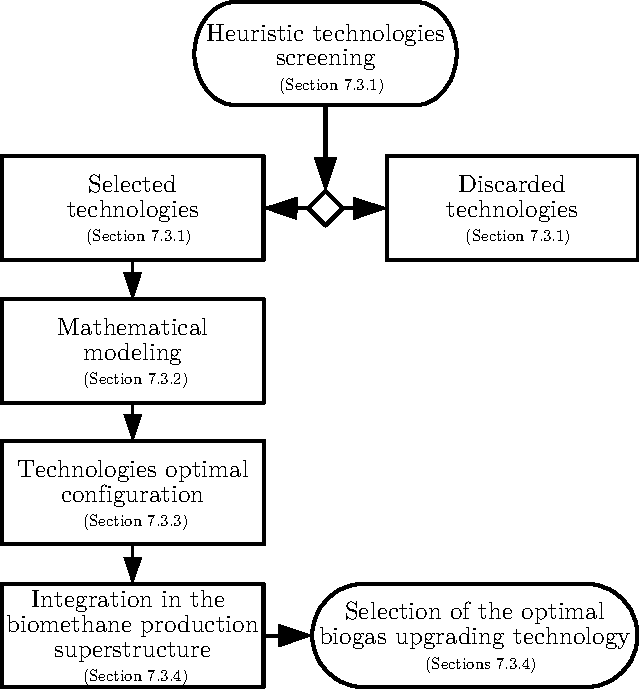
\includegraphics[width=0.8\linewidth, trim={0cm 0cm 0cm 0cm},clip]{gfx/Chapter7/Figure1.pdf} 
	\caption{Scheme of the methodology followed to determine the optimal biogas	upgrading technology.}
	\label{fig:Fig1}
\end{figure}

\begin{table}[h]
	\centering
	\caption{Characteristics of the four waste types evaluated.}
	\label{table:Ch7Table1}
	\resizebox{0.9\columnwidth}{!}{
		\begin{tabular}{@{}lcccc@{}}
			\toprule
			& \begin{tabular}[c]{@{}c@{}}Cattle \\ manure\\ \protect\citep{EuropeanCommission4953_2_11768_1}\end{tabular} & \begin{tabular}[c]{@{}c@{}}Pig\\ manure \\ \protect\citep{EuropeanCommission4953_2_11768_1,DanishEnvironmentalProtectionAgency2018}\end{tabular} & \begin{tabular}[c]{@{}c@{}}Sludge \\ (wastewater)\\ \protect\citep{EuropeanCommission4953_2_11768_1}\end{tabular} & \begin{tabular}[c]{@{}c@{}}Urban \\ food waste\\ \protect\citep{EuropeanCommission4953_2_11768_1}\end{tabular} \\ \midrule
			V\textsubscript{biogas} (m\textsuperscript{3}/kg)  & 0.25                                                                                & 0.38                                                                                            & 0.35                                                                                      & 0.44                                                                                   \\
			w\textsubscript{DM} (\% wt)       & 0.25                                                                                & 0.25                                                                                            & 0.17                                                                                      & 0.31                                                                                   \\
			w\textsubscript{VS} (\% dry wt)   & 0.80                                                                                & 0.75                                                                                            & 0.4                                                                                       & 0.85                                                                                   \\
			w\textsubscript{N} (\% dry wt)    & 0.004                                                                               & 0.006                                                                                           & 0.17                                                                                      & 0.001                                                                                  \\
			w\textsubscript{N\textsubscript{org}} (\% dry wt) & 0.020                                                                               & 0.022                                                                                           & 0.0015                                                                                    & 0.031                                                                                  \\
			w\textsubscript{P} (\% dry wt)    & 0.006                                                                               & 0.010                                                                                           & 0.035                                                                                     & 0.005                                                                                  \\
			w\textsubscript{K} (\% dry wt)    & 0.027                                                                               & 0.027                                                                                           & 0.011                                                                                     & 0.009                                                                                  \\
			R\textsubscript{CN}               & 20                                                                                  & 15                                                                                              & 15                                                                                        & 15                                                                                     \\ \bottomrule
		\end{tabular}
	}
\end{table}


\section{Process design}\label{section:Sec3}
\subsection{Technology screening}
The technologies for CO\textsubscript{2} capture considered in the model are presented in Table \ref{table:Ch7Table2}. The technologies selected after the heuristic stage are chemical absorption, PSA, and membrane separation systems. Water scrubbing is a limiting case of the use of amine solutions, where amine concentration would be zero. According to the literature the use of water scrubbing is more energy demanding, 3:1, than the use of amines \citep{Pellegrini2015}. Therefore, among scrubbing only amines will be considered. CO\textsubscript{2} hydrogenation is not actually a technology based on the removal of
the sour gas, but a transformation process that can be compared outside of the framework used in this work for the CO2 capture processes \citep{curto2019renewable}. Finally, cryogenic separation is
still under development and the costs are high \citep{adnan2019technologies}. Each of the preselected technologies shows different configurations to be selected upon:

\begin{itemize}
	\item In the case of amine scrubbing, three different amines are considered: monoethanolamine (MEA), diethanolamine (DEA), and methyl diethanolamine (MDEA) \citep{2004gpsa}.
	\item Pressure swing adsorption (PSA) systems can use different solid beds. Activated carbon presented a capture capacity about 25\% lower than zeolites 13X and 4A \citep{hauchhum2014carbon}. The material cost being similar, and the lower adsorption of	methane in the activated carbon \citep{ferella2017separation}, results in the preselection of the zeolites beds over activated carbon.
	\item Regarding the membrane systems, there are two variables to be	considered, the configuration of the membrane units, and the	material of the membranes. Among the possible configurations for the membrane units, single-stage or multi-stage arrangements can be found. Multiple stage results in larger methane recovery and lower costs \citep{deng2010techno}. Among the multiple membrane stage systems, configurations with one compression stage \citep{makaruk2010membrane} or multiple compression stages \citep{molino2013biogas} are available. According to the literature, dual-stage membrane systems with single compression stage, considering only compression before the membrane	system with no recompression stage between membrane units,	have been deemed as the most economic under a wide range of	feed compositions \citep{kim2017optimization}. Finally, the membrane materials are defined by the permeability of the gases. Lists of membrane materials for the separation of CO2 from CH4 can be	found in several reviews \citep{zhang2013modeling, chen2015membrane, vrbova2017upgrading}. Among the common materials with larger permeabilities, cellulose acetate, polyimide, and polycarbonate are considered.
\end{itemize}

\begin{table}[h]
	\centering
	\caption{CO\textsubscript{2} capture technologies considered in the study.}
	\label{table:Ch7Table2}
	\resizebox{0.8\columnwidth}{!}{
		\begin{tabular}{@{}cc@{}}
			\toprule
			CO2 capture technology    & Result after heuristic screening \\ \midrule
			Water scrubbing           & Discarded                        \\
			Amines scrubbing          & Preselected                      \\
			Pressure Swing Adsorption & Preselected                      \\
			Membranes                 & Preselected                      \\
			CO2 hydrogenation         & Discarded                        \\
			Cryogenic                 & Discarded                        \\ \bottomrule
		\end{tabular}
	}
\end{table}

\subsection{Mathematical modelling}
In this section the mathematical optimization stage of the procedure is presented and the models for the different units involved in biogas upgrading via CO\textsubscript{2} capture are described. For a more detailed description of the mathematical modelling, the reader is referred to the Supplementary Material, section \ref{section:SuppMatPaperCO2Section2}.

\subsubsection{Biogas production and conditioning} \label{section:BiogasProductionPaperBiogas}
The modelling of the biogas production and conditioning has been developed based on first principles in previous works \citet{leon2016optimal}, and therefore no further details are provided here. Anaerobic digestion is modelled based on mass and energy balances and yield data from the literature. For economic evaluation purposes, a standard digester size of 6,000 m\textsuperscript{3} is considered \citep{rohstoffe2010guia}. The biogas composition must be within the typical ratios for each of the raw materials. However, we consider it to be a variable that can be adjusted depending on its final use \citep{leon2016optimal}.

The compressors are modelled assuming polytropic behaviour, with a polytropic coefficient of 1.4, and an efficiency equal to 0.85 (Moran and Shapiro, 2003). Regarding the biogas conditioning stage, a bed of Fe\textsubscript{2}O\textsubscript{3} is used for H\textsubscript{2}S removal through the reaction described below. Experimental data shows almost 100\% removal yield for H\textsubscript{2}S using a fixed bed of Fe\textsubscript{2}O\textsubscript{3}.

\begin{align}
& \text{Fe}_{2}\text{O}_{3} + 3\text{H}_2 \text{S} \rightarrow \text{Fe}_{2}\text{S}_{3} + 3\text{H}_2 \text{O}
\end{align}

Finally, ammonia and water are removed using a PSA system, considering removal yields equal to 100\% \citep{Nexant2006, 2004gpsa}.

\subsubsection{Absorption: amines} \label{section:MathModAbsorptionAmines}
The amine scrubbing systems consist of an absorption column where the amine solution is put into contact with the biogas. The amine rich in CO\textsubscript{2} is heated up before being fed to the stripping column where the CO\textsubscript{2} is desorbed from the amine, which is recycled to the first column. The fresh amine used for making-up the losses of amine is mixed with the recycle stream from the regeneration column at the same temperature. The systems using amines typically operate at low temperatures, around 25-30 \textdegree C, and partial pressures of CO\textsubscript{2} above 0.05 bar, reaching removal yields of 90\%-95\% \citep{zhang2013modeling}. In contrast to post-combustion gases, which contain large amounts of nitrogen, biogas is composed
mainly of methane and CO\textsubscript{2}, resulting in higher carbon dioxide partial pressures requiring lower operating pressures. CO\textsubscript{2} partial pressures above 0.1 bar have been assumed to secure high removal yields \citep{zhang2013modeling}, resulting in the need to operate at total pressures around 1-1.5 bar to secure the appropriate CO\textsubscript{2} partial pressures \citep{movagharnejad2011simulation, xue2017comparative}.

Each unit is modelled based on first principles using industrial data \citep{2012gpsa}. To compute the flow of fresh amines, the CO\textsubscript{2} pickup rate and the column efficiency are used from industrial data. The energy balance to the preheater, the condenser and the reboiler of the CO\textsubscript{2} desorption column and the cooler are computed also using industrial rules of thumb. For the complete model see the Supplementary Material.

The model for the selection of the amine absorption is formulated as an NLP problem including the units described in sections \ref{section:BiogasProductionPaperBiogas} and \ref{section:SuppMatAmines} of the Supplementary Material.

\subsubsection{PSA} \label{section:MathModPSA}
The stream of gases passes through the bed of zeolites and the carbon dioxide is captured by adsorption. The system consists of the compression train and the zeolite beds. The models for each of
the units are based on the thermodynamics of gas compression and solid-gas Langmuir adsorption. The details can be seen in the Supplementary Material.

The adsorption capacity of the zeolites is directly related to the partial pressure of the CO\textsubscript{2}. Therefore, the feed pressure is an operating variable adjusted using a system of compressors with intercooling. Each compression stage is modelled assumed polytropic behaviour and a compression efficiency of 0.85. The heat exchangers are modelled using mass and energy balances so that the gas temperature is from 25 to 60 \textdegree C entering the adsorption bed. The removal yield is assumed to be 98\%, so that the exit gas contains less than 2\% CO\textsubscript{2} \citep{ferella2017separation}. The mass of zeolite depends on the adsorption capacity that is computed as a function of the operating pressure and temperature using Langmuir adsorption models for the three materials. The operating time before regeneration must be below 20 min for the product gas to contain only traces of CO\textsubscript{2} \citep{hauchhum2014carbon}. Thus, two beds operate in parallel, one in adsorption, one in desorption mode. In addition, the adsorption capacity decays cycle after cycle until it stabilizes around 65\% of the initial capacity given by Langmuir adoption isotherm. Therefore, the adsorption capacity is corrected to compute the amount of zeolite used in the PSA system. Furthermore, a lifetime of the zeolites bed of 5 years has been considered based on data reported by \citep{Xiao2013}.

The process is modelled as an NLP optimization problem including the models described in sections \ref{section:BiogasProductionPaperBiogas} and \ref{section:SuppMatPSA} of the Supplementary Material.

\subsubsection{Membranes} \label{section:MathModMembranes}
A dual-stage membrane system with single compression stage before the membrane module and no recompression stage between modules is considered since it has been deemed as the most economic arrangement under a wide range of feed compositions \citep{kim2017optimization}. The compressor is modelled as discussed above, assuming polytropic compression of the gas, see Supplementary Material for further details. Each membrane module is modelled using mass balances considering the permeate and retentate streams, the flux of the gases across the membrane, that is a function of the concentration gradient between both sides of the membrane \citep{FernandesRodriguesMsc}. The flux is the parameter which allows computing the area of the membrane, based on the permeability of the membrane. As the driving force in the membrane separation process is the concentration gradient, the
removal of CO2 results in a change in the composition of the stream along the membrane, leading to a change in the driving force which controls the process. Therefore, an average molar fraction between the feed and the retentate composition is used to compute the separation driving force. Three different membrane materials are selected aiming at large CO 2 permeability, low methane permeability, and therefore, high selectivity; cellulose acetate, polyamide, and polycarbonate \citep{vrbova2017upgrading}. The solution of the optimization problem will yield intermediate conditions to assure natural gas composition of the biomethane.

The process model is formulated as an NLP problem, including the models described in sections \ref{section:BiogasProductionPaperBiogas} and \ref{section:SuppMatMembranes} of the Supplementary Material, where the main decision variables are the operating pressure of the membrane, their areas and the flux across the membrane.

\subsection{Selection of optimal configurations}
\subsubsection{Absorption: amines}
Eq. \ref{eq:Ch7Eq1} and the objective function shown in Eq. \ref{eq:Ch7Eq2} are added to the model described in section \ref{section:MathModAbsorptionAmines} for determining the optimal amine for biogas upgrading. The first term, BioCH4, presents the profit from the biomethane generated using the price of the natural gas given by \citet{EIAPrices}, and the second term corresponds to the operation considering the amortization of the investment costs of the amines purification systems, calculated in Eq. \ref{eq:Ch7Eq2}, where the investment cost is annualized with K equal to 3 \citep{douglas1988conceptual}.

\begin{align}
	& Profit_{{Amine \ system}} = BioCH_{4} - Cost_{{Amine \ system}} \label{eq:Ch7Eq1}\\
	& Cost_{{Amine \ system}} = \nonumber \\
	& C_{{Steam}}\sum\limits_i \frac{Q_i}{\lambda} \cdot \tau _{{year}} + \frac{1}{K} C_{{Amine}}\cdot fc_{{Amine}} \cdot \tau _{{year}} \label{eq:Ch7Eq2}
\end{align}

The cost of each amine is taken to be 1.3 USD/kg for MEA, 1.32 USD/kg for DEA, and 3.09 USD/kg for MDEA, based on \citet{nuchitprasittichai2013optimization}. The cost of high pressure steam (42 bar) is assumed to be 0.019 USD/kg \citep{perez2019superstructure}. The NLP problem consists of 288 equations and 953 variables per amine evaluated and is solved using a multistart initialization approach with CONOPT as the preferred solver where the main decision variables are the pressures temperatures and flow rates.

\subsubsection{PSA}
The main decision variables to select among the zeolite materials are the operating pressure and temperature at the PSA bed and the size of the zeolites bed. To estimate the cost of the PSA system, Eqs. \ref{eq:Ch7Eq3} and \ref{eq:Ch7Eq4} are included in the model described in section \ref{section:MathModPSA}, assuming that the zeolite bed loses efficiency over time, resulting in a lifetime of 5 years before it needs to be replaced \citep{Xiao2013}. As the plant life is considered to be 20 years, the zeolites bed must be replaced 4 times during the plant life, N Cycle. The cost of the zeolites considered is 5 USD/kg for both, zeolite 13 X and zeolite 4A \citep{Xiao2013}.

\begin{align}
& Profit_{{PSA \ system}} = BioCH_{4} - Cost_{{PSA \ system}} \label{eq:Ch7Eq3}
\end{align}

\begin{align}
& Cost_{{PSA \ system}} =  \label{eq:Ch7Eq4} \\
& C_{Electricity} \cdot W_{{Compressor}} + \frac{1}{K} M_{{Zeolite}}\cdot C_{{Zeolite}}\cdot N_{{Cycle}} \nonumber
\end{align}

The NLP problems, consisting 283 equations and 828 variables per adsorbent material, are solved similarly as in the case of the selection of amines.

\subsubsection{Membranes}
The selection of membrane material is carried out using the model described in \ref{section:MathModMembranes}, and an objective function considering the cost of the gas compression and the amortization of the investment costs of the membranes, Eqs. \ref{eq:Ch7Eq5} and \ref{eq:Ch7Eq6}.

\begin{align}
Profit_{Membrane \ system} = BioCH_{4}- Cost_{{Membrane \ system}} \label{eq:Ch7Eq5}
\end{align}

\begin{align}
& Cost_{{Membrane \ system}} = \label{eq:Ch7Eq6} \\
& {C}_{Electricity} \cdot W_{Compressor} + \frac{1}{K} \cdot C_{Membrane} \cdot \frac{1}{Lf} \nonumber \\
& \cdot N_{Membranes} \left(\sum\limits_{i \in stages} {Area_i}\right) \nonumber
\end{align}

A value of 50 USD/m\textsuperscript{2} will be used based on the literature \citep{kim2017optimization}. Considering the plant life equal to 20 years, the membranes with a typical lifetime of 4 years must be replaced 5 times during the plant life, $N_{Membranes}$ \citep{scholz2015structural}. Each NLP consists of 299 equations and 869 variables and it is solved as the ones formulated for the previous cases.

\subsection{Superstructure configuration}\label{section:SuperstructureConfiguration}
Once the best configuration from each technology is selected, the superstructure containing all the technologies evaluated is built considering only the best amine, membrane material and adsorbent bed, see Fig. \ref{fig:Ch7Fig2}. The superstructure includes the models presented in sections \ref{section:BiogasProductionPaperBiogas} to \ref{section:MathModMembranes} and described in the Supplementary Material, section \ref{section:SuppMatPaperCO2Section2}. The superstructure is optimized evaluating all the processes simultaneously, for each waste raw material selecting only one technology, using as objective function Eq. \ref{eq:Ch7Eq7}.

\begin{align}
& Profit = \label{eq:Ch7Eq7}  \\
& BioCH_{4} - Cost_{{Membrane \ system}} - Cost_{{PSA \ system}} - Cost_{{Amine \ system}} \nonumber
\end{align}

The superstructure model consists of 383 equations and 1367 variables, resulting in an NLP problem solved using a multistart optimization procedure with CONOPT as the preferred solver. The main decision variables are operating conditions including flows, temperatures, pressures, whereas the value for the variables of the non-selected technologies is null, including the mass flow. Binary
variables per technology are not needed for the selection among the technologies since the costs are related to the flow processed per each technology.

\begin{figure}[h]
	\centering
	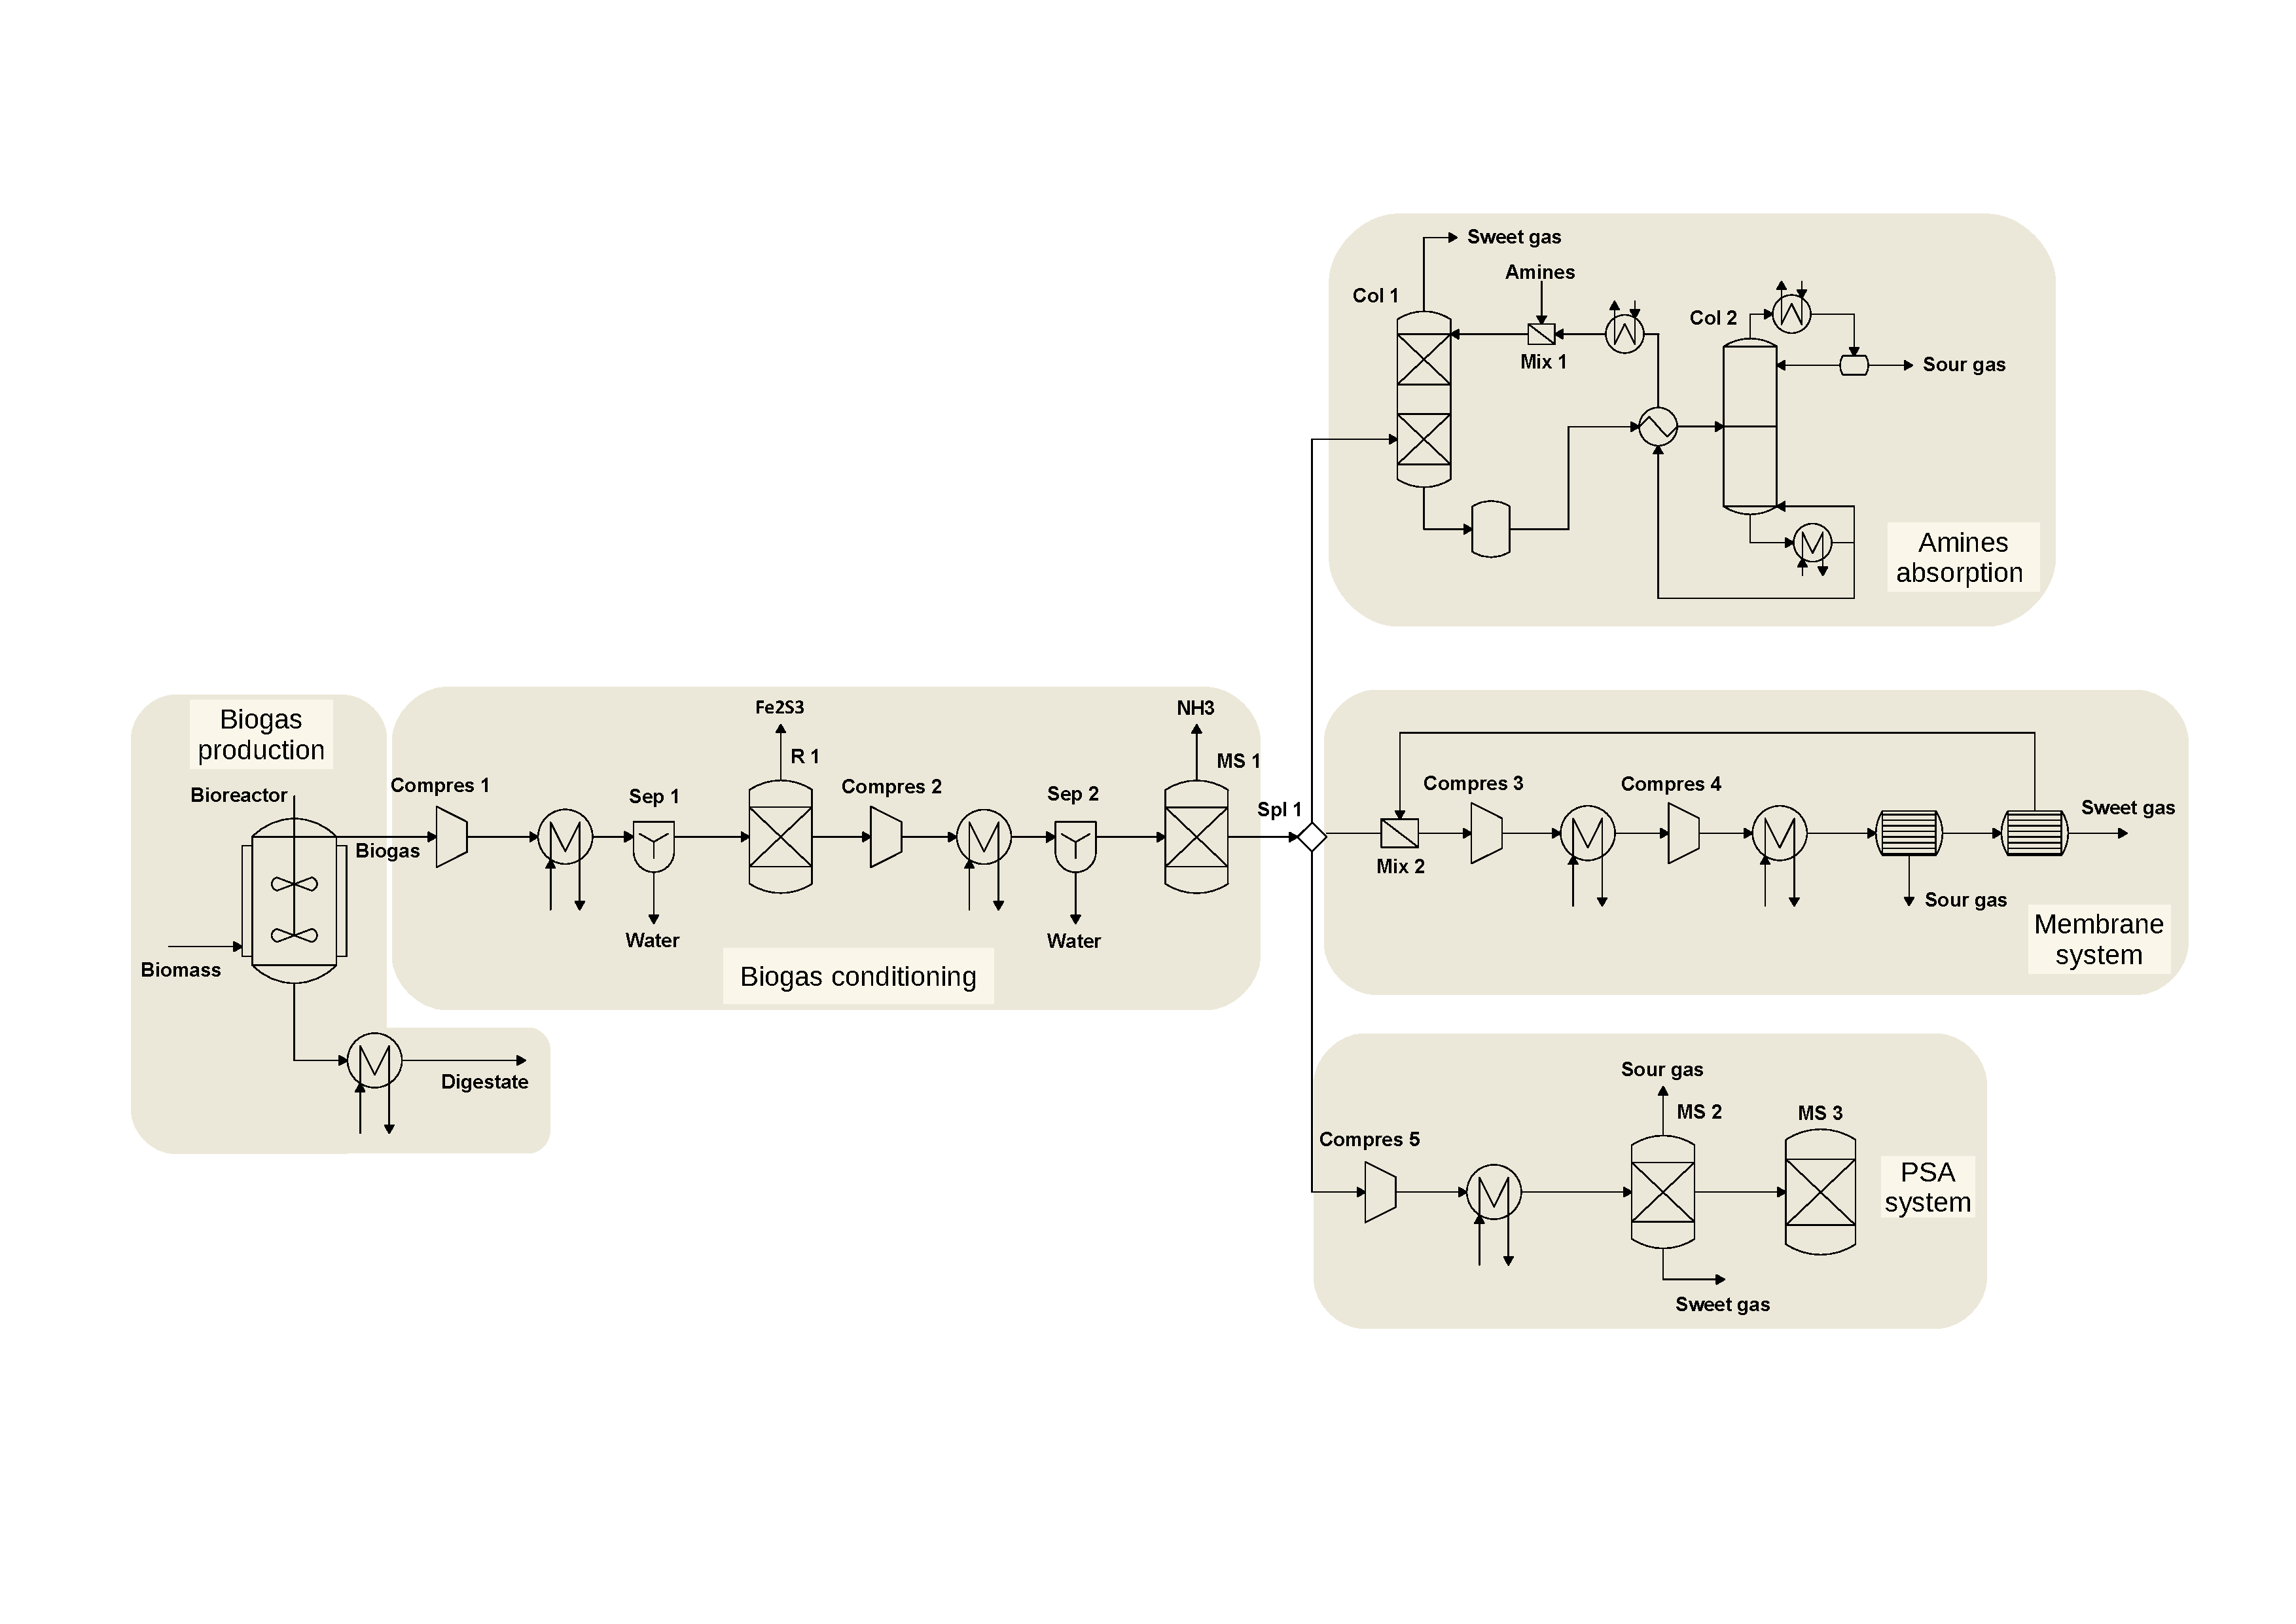
\includegraphics[width=1\linewidth, trim={3cm 7cm 3cm 5cm},clip]{gfx/Chapter7/Figure2.pdf} 
	\caption{Scheme of the proposed superstructure for biogas upgrading into biomethane.}
	\label{fig:Ch7Fig2}
\end{figure}

\subsection{Economic evaluation}\label{section:Ch7Economicevaluation}
Finally, a detailed economic evaluation for biomethane production from different wastes is performed. The production and investment costs are estimated using the factorial method presented in \citet{towler2009chemical}. It is based on the estimation of the unit costs, using the same factors as presented in \citet{davis2014optimala, davis2014optimalb} for further comparison with other renewable based methane production processes. The details on the method and correlations used for the economic assessment can be seen in the Supplementary Material, section \ref{section:SuppMatPaperCO2Section3}.


\section{Results}\label{section:Sec4}
This section draws the results for the composition of the biogas obtained, technology selection, economic evaluation, the comparison of different technologies beyond biogas upgrading for the production of biomethane, and a scale-up study.

\subsection{Biogas composition}
The amount of each component of biogas is not fixed, but limited by upper and lower bounds for each component, as a range of values provided by the literature. The model aims at the composition of biogas that optimizes the production of methane, resulting in the same composition for all wastes, shown in Table \ref{table:Ch7Table3}.

\begin{table}[h]
	\centering
	\caption{Raw biogas composition.}
	\label{table:Ch7Table3}
	\resizebox{\columnwidth}{!}{
		\begin{tabular}{@{}cccccccc@{}}
			\toprule
			& CH\textsubscript{4}  & CO\textsubscript{2}  & H\textsubscript{4}S  & NH\textsubscript{3}        & N\textsubscript{2}  & O\textsubscript{2}  & H\textsubscript{2}O  \\ \midrule
			Biogas composition (\% mol) & 56.8 & 25.2 & $\leq$0.2 & $\leq 7.6 \cdot 10^{-3}$ & 1.7 & 0.4 & 15.7 \\ \bottomrule
		\end{tabular}
	}
\end{table}

\subsection{Selection of technology}
This section is divided into the selection of the best configuration per preselected technology and the optimization of the operating conditions where an economic objective function has been considered.

\subsubsection{Selection of the optimal configuration}
The selection of the optimal configuration of each technology, amines, PSA and membranes is carried out in a first optimization stage. Since the composition turned out to be the same for all wastes, the selection of technologies was also the same for the four wastes. In the case of the amines, DEA is the best among the amines. Note that the prices for the different amines change, but the recycle of the amines is such that the largest share of the cost comes from the energy involved in the regeneration column. Regarding adsorbent beds, zeolite 13 X shows the largest adsorption capacity. Finally, polyimide results as the best membrane material.

\subsubsection{Selection of the optimal technology and operating conditions}
The selection of technology for biogas upgrading was performed for four different wastes: cattle and swine manure, municipal food waste and sludge. The biogas upgrading technology selected for all
residues is pressure swing adsorption. The results of the optimization problem formulated returns the optimal operating conditions of the biomethanation production facility for the wastes evaluated, as shown in Table \ref{table:Ch7Table4}. Regarding the wastes studied, food waste is the most promising one for biomethane production due to the larger organic matter content.

\begin{table}[h]
	\centering
	\caption{Main process parameters for the selected technology, pressure swing adsorption.}
	\label{table:Ch7Table4}
	\resizebox{\columnwidth}{!}{
		\begin{tabular}{@{}ccccc@{}}
			\toprule
			& Food waste   & Cattle manure & Pig manure  & Sludge      \\ \midrule
			Waste flow (kg/s)                & 9.795        & 9.795         & 9.795       & 9.795       \\
			kg methane/kg feed               & 0.0355       & 0.00826       & 0.00449     & 0.00929     \\
			\begin{tabular}[c]{@{}c@{}}Methane produced \\ ($10^{-6}$ Nm\textsuperscript{3}/yr)\end{tabular}  & 15.132       & 3.521         & 1.914       & 3.960       \\
			P\textsubscript{PSA} (atm)                      & 2            & 2             & 2           & 2           \\
			T\textsubscript{PSA} (\textdegree C)                       & 25           & 25            & 25          & 25          \\
			M\textsubscript{Zeolite} (kg)                 & 6835         & 1583          & 856         & 1781        \\
			Steam (MW)                       & 4.2          & 3.7           & 3.3         & 4.9         \\
			Cooling (MW)                     & 3.3          & 0.7           & 0.4         & 1.0         \\
			Power (kW)                       & 223          & 51.2          & 28          & 58.0        \\
			NPK ratio                        & 1.1/0.9/0.47 & 1.1/1.1/0.6   & 0.8/2.5/1.3 & 0.0/4.6/2.4 \\
			R\textsubscript{CN}                             & 13.7         & 21.0          & 7.8         & 14.8        \\ \bottomrule
		\end{tabular}
	}
\end{table}

\subsection{Estimation of production and investment costs}
Table \ref{table:Ch7Table5} shows the summary of the results of the economic evaluation considering the best upgrading technology for the different raw materials evaluated, and Fig. \ref{fig:Ch7Fig3} presents the break-down of the production costs. Food waste is the most competitive residue for biomethane production, resulting in a production cost of 0.36 EUR/Nm3. One the other hand, the low organic load in manure results in production costs from 3 to 5 times larger than the production cost of biomethane from food waste. In all cases, the production cost is higher than current natural gas costs (0.18 EUR/Nm3) \citep{EIAPrices} by at least a factor of 2. Therefore, the NPV or the ROI would be negative resulting in the need for additional income to balance the production costs obtaining credit from the nutrients contained within digestate, or through the application of incentive policies resulting in competitive market prices for biomethane. Considering the first alternative, food waste based biomethane, the most favourable case, becomes competitive if a credit of 0.022 EUR per kilogram of the fertilizer is obtained considering a methane market value of 5 EUR/MMBTU (0.18 EUR/Nm3), while the more expensive biomethane, obtained from swine manure, can be competitive at the cost of 0.116 EUR/kg of fertilizer. Considering a feed-in premium (FiP) incentive scheme, where bonuses are paid above the benchmark market price to subsidize the biomethane production, a range of bonus values between the 100\% and 1000\% of the methane market value are needed to reach a competitive selling price.

\begin{figure}[h]
	\centering
	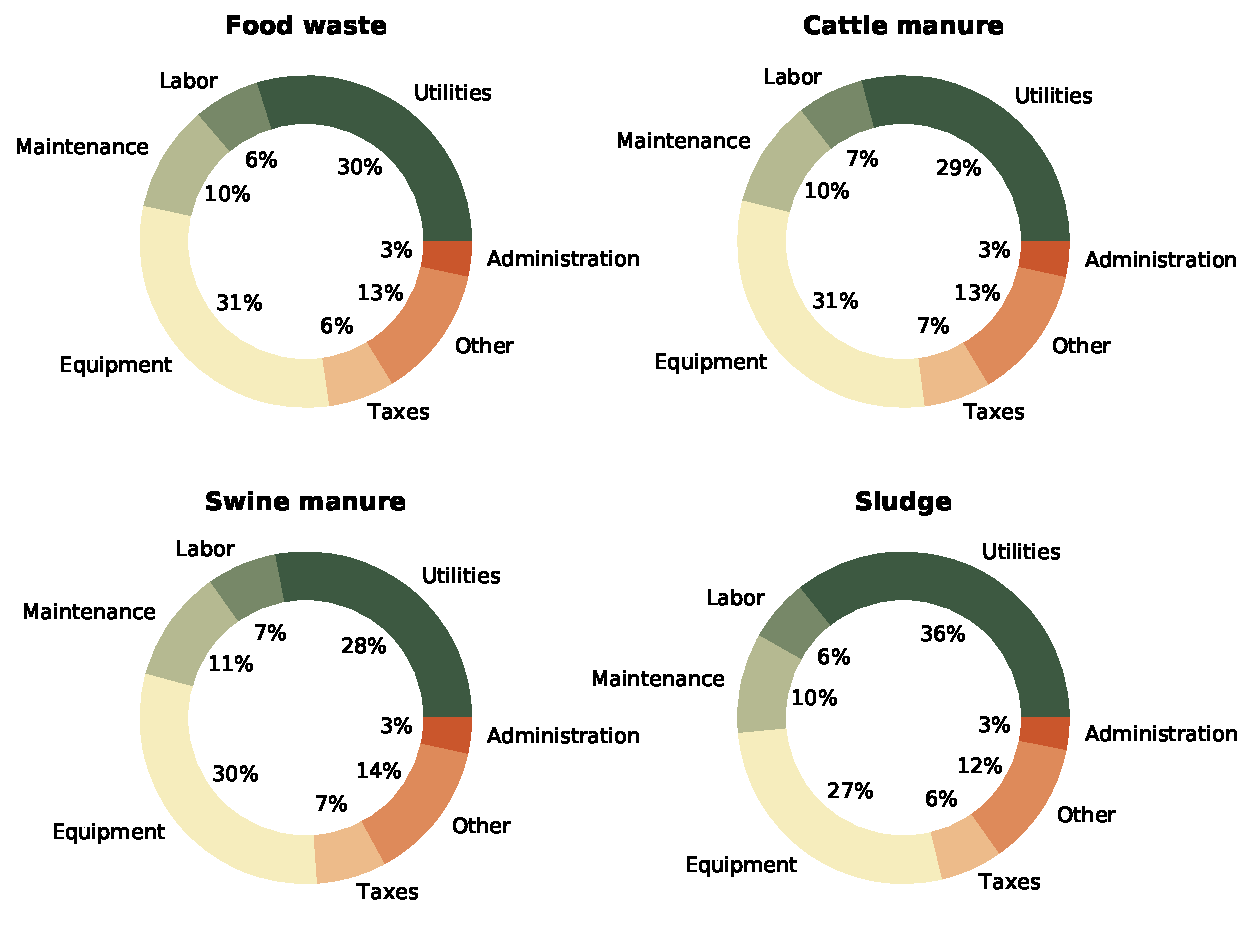
\includegraphics[width=1\linewidth, trim={0cm 0cm 0cm 0cm},clip]{gfx/Chapter7/Figure3.pdf} 
	\caption{Breakdown of biomethane production costs for each residue analyzed.}
	\label{fig:Ch7Fig3}
\end{figure}

Regarding investment costs, the processing of larger flows of biogas for the processing of food waste results in up to 25\% larger investment costs, from 49 M EUR to 66 M EUR, although as the flows of raw
waste are similar for the different residues evaluated the number of digesters required is the same.

For the most promising waste towards biomethane production, food municipal waste, the production and investment costs are computed in detail for the selected technologies, namely, PSA, membranes and amines, as shown in Table \ref{table:Ch7Table6}. It is possible to see that membranes and PSA show similar economic results, slightly in favour of the first technology. Membrane systems requires 3 times more power than PSA units, resulting in a slightly more expensive alternative than the PSA. The optimal operating pressure of membranes is 65 bar, in the order of that presented by \citet{kim2017optimization}, while the pressure of the PSA system is 2.05 bar, according with the results reported in \citep{ferella2017separation} for biogas upgrading, and in the lower bound of the operating conditions reported by \citet{santos2011pressure}. Amines scrubbing results the most expensive upgrading technology resulting in a cost 10\% higher, mainly due to the larger consumption of utilities in the form of steam for the regeneration of the solvent. In all cases, with a reasonable credit from the fertilizer it would be possible to produce biomethane at a competitive cost, while the FiP bonus are between 100\% and 117\% of the methane market value.

\begin{table}[h]
	\centering
	\caption{Summary of the cost estimation for biomethane production considering the optimal biogas upgrading technology, PSA system.}
	\label{table:Ch7Table5}
	\resizebox{\columnwidth}{!}{
		\begin{tabular}{@{}ccccc@{}}
			\toprule
			& Food Waste                                                             & Cattle Manure                                                         & Pig Manure                                                             & Sludge                                                                 \\ \midrule
			N\textdegree of digesters                                                                    & 6                                                                      & 6                                                                     & 6                                                                      & 6                                                                      \\
			Investment cost (M EUR)                                                            & 66.4                                                                   & 54.4                                                                  & 48.7                                                                   & 51.3                                                                   \\
			Production cost (M EUR/yr)                                                         & 5.1                                                                    & 4.0                                                                   & 3.6                                                                    & 4.2                                                                    \\
			Production cost (no credit)                                                        & \begin{tabular}[c]{@{}c@{}}0.36 $\frac{\text{EUR}}{\text{Nm}^3}$ \\ 10.0 $\frac{\text{EUR}}{\text{MMBTU}}$\end{tabular} & \begin{tabular}[c]{@{}c@{}}1.24 $\frac{\text{EUR}}{\text{Nm}^3}$\\ 33.5 $\frac{\text{EUR}}{\text{MMBTU}}$\end{tabular} & \begin{tabular}[c]{@{}c@{}}2.00 $\frac{\text{EUR}}{\text{Nm}^3}$ \\ 55.4 $\frac{\text{EUR}}{\text{MMBTU}}$\end{tabular} & \begin{tabular}[c]{@{}c@{}}1.15 $\frac{\text{EUR}}{\text{Nm}^3}$ \\ 31.8 $\frac{\text{EUR}}{\text{MMBTU}}$\end{tabular} \\
			\begin{tabular}[c]{@{}c@{}}EUR/kg fertilizer to\\ achieve 5 EUR/MMBTU\end{tabular} & 0.022                                                                  & 0.048                                                                 & 0.116                                                                  & 0.041                                                                  \\
			\begin{tabular}[c]{@{}c@{}}EUR/Nm\textsuperscript{3} FiP bonus to\\ achieve 5 EUR/MMBTU\end{tabular} & 0.18                                                                   & 1.029                                                                 & 1.819                                                                  & 0.97                                                                   \\ \bottomrule
		\end{tabular}
	}
\end{table}

\begin{table}[h]
	\centering
	\caption{Detailed analysis for production of biomethane from food waste comparing technologies.}
	\label{table:Ch7Table6}
	\resizebox{0.85\columnwidth}{!}{
		\begin{tabular}{@{}cccc@{}}
			\toprule
			& \multicolumn{3}{c}{Food Waste}                                                                                                                                                                                        \\ \midrule
			& PSA                                                                   & Membranes                                                             & Amines                                                                \\
			Waste flow (kg/s)                        & 9.795                                                                 & 9.795                                                                 & 9.795                                                                 \\
			Kg Methane/kg feed                       & 0.0355                                                                & 0.0355                                                                & 0.0355                                                                \\
			N\textdegree of digesters                          & 6                                                                     & 6                                                                     & 6                                                                     \\
			Steam (MW)                               & 4.2                                                                   & 4.2                                                                   & 6.1                                                                   \\
			Cooling (MW)                             & 3.3                                                                   & 3.4                                                                   & 5.0                                                                   \\
			Power (kW)                               & 223                                                                   & 665                                                                   & 145                                                                   \\
			Investment cost (M EUR)                  & 66.4                                                                  & 65.2                                                                  & 67.1                                                                  \\
			Production cost (M EUR/yr)               & 5.1                                                                   & 5.3                                                                   & 5.7                                                                   \\
			Production cost (no credit)              & \begin{tabular}[c]{@{}c@{}}0.36 $\frac{\text{EUR}}{\text{Nm}^3}$\\ 10.0 $\frac{\text{EUR}}{\text{MMBTU}}$\end{tabular} & \begin{tabular}[c]{@{}c@{}}0.38 $\frac{\text{EUR}}{\text{Nm}^3}$\\ 10.5 $\frac{\text{EUR}}{\text{MMBTU}}$\end{tabular} & \begin{tabular}[c]{@{}c@{}}0.39 $\frac{\text{EUR}}{\text{Nm}^3}$\\ 10.7 $\frac{\text{EUR}}{\text{MMBTU}}$\end{tabular} \\
			\begin{tabular}[c]{@{}c@{}}EUR/kg fertilizer to\\ achieve 5 EUR/MMBTU\end{tabular} & 0.022                                                                 & 0.023                                                                 & 0.026                                                                 \\
			\begin{tabular}[c]{@{}c@{}}EUR/Nm\textsuperscript{3} FiP bonus to\\ achieve 5 EUR/MMBTU\end{tabular} & 0.18                                                                  & 0.20                                                                  & 0.21                                                                  \\ \bottomrule
		\end{tabular}
	}
\end{table}

\subsection{Comparison with renewable-based hydrogenation processes}
The results presented in this work are compared with two different technologies for renewable methane production, the hydrogenation of the CO\textsubscript{2} contained in the biogas, reported by \citet{curto2019renewable}, and synthetic methane produced from CO\textsubscript{2} hydrogenation, as presented by \citet{davis2014optimala, davis2014optimalb}. In both cases, renewable energy is used to produce hydrogen, resulting in a high dependency between the methane production cost and the local availability of the renewable energy sources, i.e. solar irradiance and wind.

For the hydrogenation of the CO\textsubscript{2} within the biogas, the production costs depend on the mode of operation, continuum production or variable with the availability of solar energy. Considering a facility for food waste processing, with a production capacity of 0.67 kg/s of biomethane, a range of production costs of 0.57-0.27 EUR/Nm3 for CO\textsubscript{2} hydrogenation under steady and varying conditions respectively is found, with investment costs of 229 M EUR and 116 M EUR for the same two operating modes in Spain \citep{curto2019renewable}.

Alternatively, direct hydrogenation of CO\textsubscript{2} also allows the production of methane. For a facility with a methane production capacity of 0.78 kg/s, considering wind-based energy located in the most favourable allocation in Spain an investment of 375 M EUR is required. The production cost of synthetic methane is 0.48 EUR/Nm3, equivalent to 13.1 EUR/MMBTU (Davis and Martín, 2014a). On the other hand, if solar is used as source of renewable energy, the investment and production costs are reduced to 240 M EUR and 0.33 EUR/m3 (9.2 EUR/MMBTU) respectively in normal climate conditions \citet{davis2014optimalb}.

However, the comparison is not straightforward due to two reasons: the economies of scale and the effect of the credits obtained from digestate. The comparison can be carried out based on the feed flowrate, as in all cases a flow of waste of 10 kg/s is considered. Alternatively, the facility presented in this work is scaled-up to reach a similar methane production capacity. However, the difficulty of determining the correct credit obtained from the digestate makes difficult the direct comparison of biomethane/methane production costs.

\subsubsection{Comparison based on feed flowrate}
By comparing facilities that process the same waste flowrate, see Table \ref{table:Ch7Table6}, to the ones reported in the previous two paragraphs, the investment costs are lower in case of biogas upgrading using carbon capture technologies. The production of biomethane via CO\textsubscript{2} capture can be more competitive than the processes based on hydrogenation of CO\textsubscript{2} within the biogas except if the production rate is allowed to follow the availability of renewable energy. In addition, CO\textsubscript{2} capture is more attractive than the direct hydrogenation of CO\textsubscript{2} using wind as energy source for the production of the hydrogen, and only slightly more expensive than using solar energy. However, the biomethane production capacity is the lowest of all three processes. Furthermore, note that allocations with favourable wind and solar based hydrogen production were selected.

\subsubsection{Comparison based on production capacity}
By scaling up the facility presented in this work, just for food residues and the best technology, the PSA, the production capacity is doubled reaching 0.72 kg/s of methane for comparison with previous work. This production capacity is between the two alternatives presented above \citep{curto2019renewable,davis2014optimala,davis2014optimalb}. The economic results for the scale-up of the carbon capture facility processing food are shown in Table \ref{table:Ch7Table7} where it can be observed that the investment cost is in between the value obtained for continuum operation and the value obtained for variable hydrogenation of the CO\textsubscript{2} within the biogas. The production cost of the scaled-up facility is promising, 0.30 EUR/Nm3. Comparing this value with the ones from biogas hydrogenation or direct CO\textsubscript{2} hydrogenation, it is possible to observe that the production costs are competitive, and can be even lower than those of both technologies if a credit from the digestate can be obtained. The one drawback of the facility that uses carbon capture technologies is the need to find a use to the captured CO\textsubscript{2}. The advantage is that it does not require additional power to produce renewable hydrogen.

Therefore, the recommendation among biogas upgrading via CO\textsubscript{2} capture, via CO\textsubscript{2} hydrogenation or synthetic methane production, would depend on the availability of solar or wind energy. Considering the case of Spain, the use of variable production of methane with the solar energy by direct hydrogenation of the CO2 contained in the biogas is the best alternative \citep{curto2019renewable}. However, this is only competitive in the south of the country. Renewable methane can be the alternative when the power is produced in regions of high wind velocity \citep{de2016characterization}. Otherwise, the use of CO\textsubscript{2} capture technologies is preferred.

\begin{table}[h]
	\centering
	\caption{Operating conditions and economic parameter for the scaled-up plant from food waste.}
	\label{table:Ch7Table7}
	\resizebox{0.55\columnwidth}{!}{
		\begin{tabular}{@{}cc@{}}
			\toprule
			& Food Waste                                                            \\ \midrule
			kg Methane/kg feed                                                               & 0.72/20                                                               \\
			N\textdegree of digesters                                                                  & 12                                                                    \\
			Investment cost (M EUR)                                                          & 124.5                                                                 \\
			Production cost (M EUR/yr)                                                       & 8.6                                                                   \\
			Credit digestate (M EUR/yr)                                                      & 38.3                                                                  \\
			Production cost (no credit)                                                      & \begin{tabular}[c]{@{}c@{}}0.30 $\frac{\text{EUR}}{\text{Nm}^3}$\\ 8.21 $\frac{\text{EUR}}{\text{MMBTU}}$\end{tabular} \\
			\begin{tabular}[c]{@{}c@{}}EUR/kg fertilizer to\\ achieve 5 EUR/MMBTU\end{tabular} & 0.014                                                                 \\ \bottomrule
		\end{tabular}
	}
\end{table}

\subsection{Plant scale-up study}
Economies of scale play an important role in the chemical industry, reducing the cost as the facilities are larger. Because of the distributed availability of the residues and the difficulty of transport, it is relevant to evaluate the effect of the scale on the process economics. Two of the four residues, food waste and cattle manure, are considered for further analysis due to the large amounts of wastes produced and the environmental concerns involved. In the first case the aim is to evaluate the cost for the biomethane for different city sizes as a function of the residues that they collect. Cities from 50 k to 5 million habitants are considered using the waste production rates of Spain, as shown in Fig. \ref{fig:Ch7Fig4}. Similar relationship between population and food waste generated can be expected for other countries or regions with a similar development level, although the results can be slightly affected by variations of some parameters, such as the amount of waste generated per person per year and the distribution of the population between urban and rural areas. The second case of study corresponds to cattle manure, assessing the biomethane production cost as a function of the size of concentrated animal feeding operations (CAFOs), considering facilities up to 16.000 cows. For a detailed description of the procedure followed in the scale-up study we refer the reader to the section S4 of the Supplementary Material. The cost of each unit is modelled as a function of the size, which is related to the mass or energy flow, as presented in the section \ref{section:SuppMatPaperCO2Section4} of the Supplementary Material. The investment and production costs are estimated as described in section \ref{section:Ch7Economicevaluation}. Fig. \ref{fig:Ch7Fig5} shows the production and investment costs as a function of the city size, and Fig. \ref{fig:Ch7Fig6} shows the scale-up for cattle manure.

\begin{figure}[h]
	\centering
	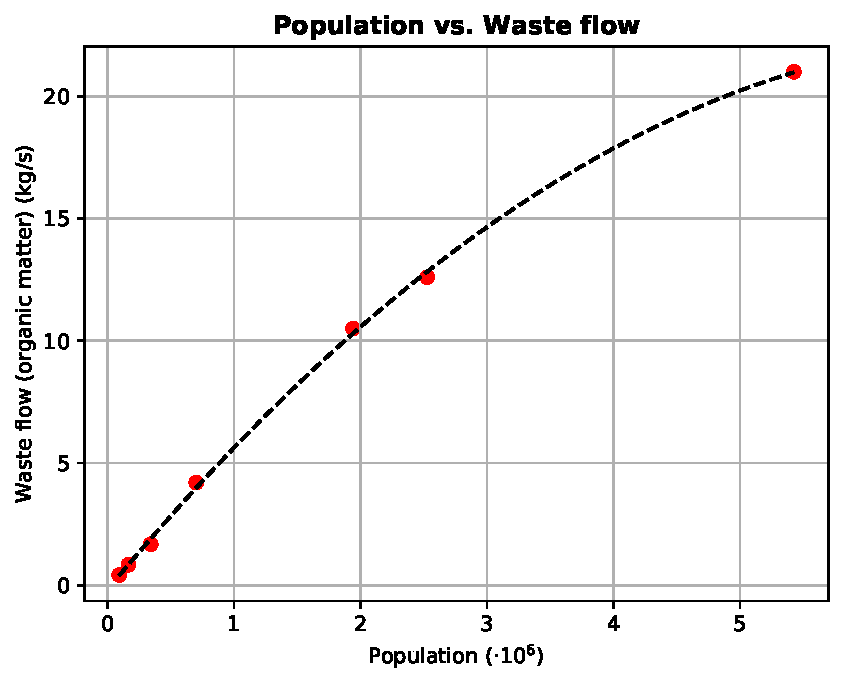
\includegraphics[width=0.8\linewidth, trim={0cm 0cm 0cm 0cm},clip]{gfx/Chapter7/Figure4.pdf} 
	\caption{Relation between population and food waste produced in Spain.}
	\label{fig:Ch7Fig4}
\end{figure}

The results show that large cities above 1 million inhabitants are able to produce biomethane at competitive prices, even more if credit is obtained from the digestate. However, the lower concentration of organic matter in cattle manure results in non-competitive prices for the biomethane produced even for the largest CAFOs considered. Therefore, manure digestion can be a way to self-produce energy, particularly in isolated places, but at larger cost. After the scale-up study we correlated the investment and production costs of biomethane as a function of the plant size. The fitting parameters for the correlations can be found in Table \ref{table:Ch7Table8}.

\begin{figure}[h]
	\centering
	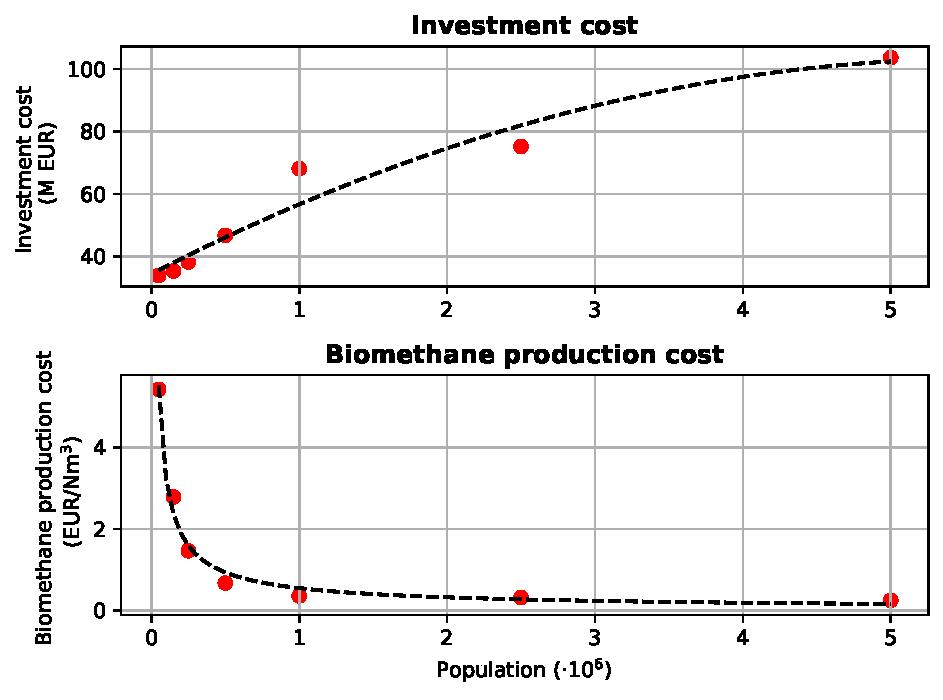
\includegraphics[width=0.9\linewidth, trim={0cm 0cm 0cm 0cm},clip]{gfx/Chapter7/Figure5.pdf} 
	\caption{Scale-up in the investment costs for municipal food waste.}
	\label{fig:Ch7Fig5}
\end{figure}

\begin{figure}[h]
	\centering
	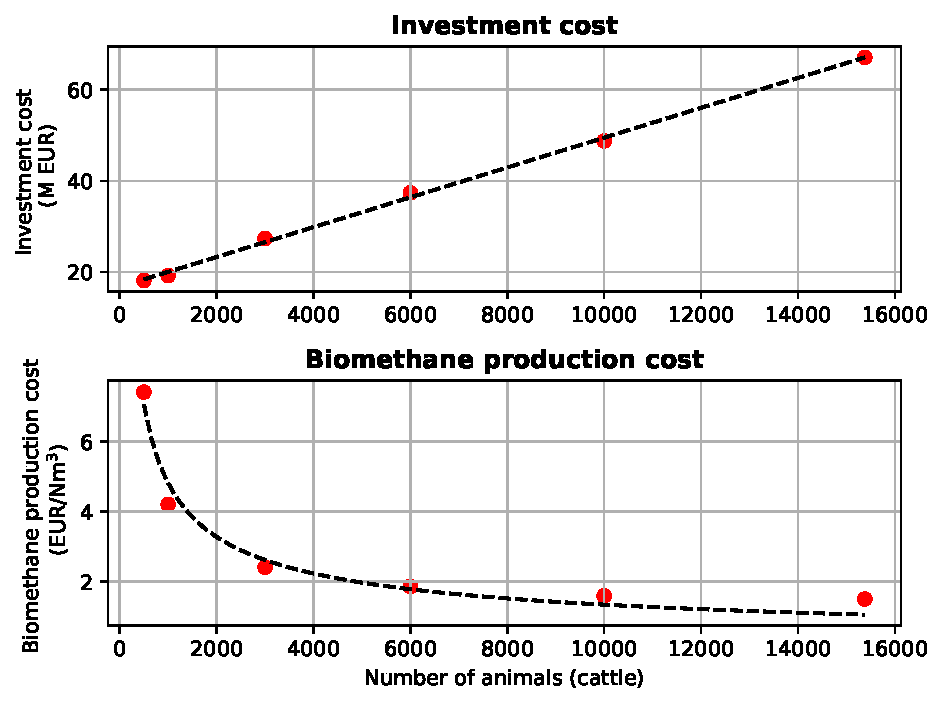
\includegraphics[width=0.9\linewidth, trim={0cm 0cm 0cm 0cm},clip]{gfx/Chapter7/Figure6.pdf} 
	\caption{Scale-up in the investment costs for cattle manure.}
	\label{fig:Ch7Fig6}
\end{figure}

\begin{table}[h!]
	\centering
	\caption{Scale-up correlations for investment and production costs for food waste and cattle manure.}
	\label{table:Ch7Table8}
	\resizebox{\columnwidth}{!}{
		\begin{tabular}{@{}cccc@{}}
			\toprule
			& Correlation         & Food Waste                               & Cattle                             \\ \cmidrule(l){3-3} \cmidrule(l){4-4}
			&                     & \small$V=\text{Population} \cdot 10^{-6}$          & \small$V=\text{Number of animals} \cdot 10^{-6}$    \\ \midrule
			Waste flow (kg/s)         & $F=a\cdot V^2 + b \cdot V + c$ & \begin{tabular}[c]{@{}c@{}}$a=-0.430$ \\ $b = 6.231$ \\ $c=-0.175$\end{tabular}  &                                    \\ \midrule
			Investment (MV)           & $I=a\cdot V^2 + b \cdot V + c$  & \begin{tabular}[c]{@{}c@{}}$a = -2.173$ \\ $b = 24.485$ \\ $c = 34.325$\end{tabular}  & \begin{tabular}[c]{@{}c@{}}$a = 0$ \\ $b = 0.003$ \\ $c = 16.769$\end{tabular} \\ \midrule
			\begin{tabular}[c]{@{}c@{}}Production costs\\ (EUR/Nm\textsuperscript{3})\end{tabular}  & $C=a\cdot V^b$        & \begin{tabular}[c]{@{}c@{}}$a = 0.546$ \\ $b = -0.771$\end{tabular}               & \begin{tabular}[c]{@{}c@{}}$a = 220.023$ \\$b = -0.553 $\end{tabular}       \\ \bottomrule
		\end{tabular}
	}
\end{table}

\section{Conclusions}\label{section:Sec5}
In this work the upgrading of the biogas produced from different waste sources is studied comparing different carbon capture technologies following a systematic framework. A hybrid heuristic-mathematical approach is developed for the systematic process design. The heuristic screening stage based on literature data is used to narrow the search. Next, a mathematical optimization approach is used to compare the most promising technologies and determine their operating conditions from an economic point of view. The framework is flexible to include more alternatives and compare novel technologies for different wastes, but relies on the prediction capacity of the models. The study evaluated swine and
cattle manure, food solid waste and sludge.

The heuristic screening suggests the use of amine scrubbing, PSA adsorption, and membrane separation systems. Within each one of them, different configurations are evaluated, focusing on the study of different amines, including MEA, DEA, and MDEA, different membranes, including polycarbonate, polyimide, and cellulose acetate, and two types of zeolites for PSA systems, 13X and 4A. The selection of the best configuration for each technology is carried out formulating and solving an optimization problem for each
technology. DEA, zeolite 13X and polyimide are the alternative selected. Next, a superstructure is formulated as an optimization problem for the processing of food waste, cattle manure, swine manure, and sludge, assessing the upgrading technologies for the production of high purity biomethane. The optimal technology for CO\textsubscript{2} capture for all residues studied is PSA systems with zeolite 13X as adsorbent material, although the use of membranes is just slightly more expensive. A detailed economic evaluation is performed for the entire biomethane production plant, yielding the production and investment costs for the production of biomethane. Food waste is the most promising waste due to the largest organic matter, resulting in an investment cost of 67 M EUR and a production cost of 0.36 EUR/Nm3 for the processing of 10 kg/s of waste. Finally, the upgrading of biogas using CO\textsubscript{2} capture is compared to direct CO\textsubscript{2} hydrogenation and direct production of synthetic methane. The comparison is in favour of the direct hydrogenation of CO\textsubscript{2}, although this result is highly dependent on the availability of solar or wind energy. For low availabilities of these resources, biomethane production through CO\textsubscript{2} capture is suggested.

This framework is of general use of the systematic evaluation of technologies and can be extended for comparison of newly developed materials and technologies as well as the evaluation of different wastes. Life cycle assessment (LCA) can be added for a multiobjective kind of optimization beyond the production cost aiming at the most sustainable production of biomethane.


\section*{Nomenclature}
\addcontentsline{toc}{section}{Nomenclature}

%{\color{red}{CHECK IF ALL THESE VARIABLES APPEAR IN THE CHAPTER}}
\vspace{-0.8cm}
\begingroup     
\let\clearpage\relax
%
\newglossaryentry{Ch7var1}{type=VarCh7,name={$A$},description={Antoine equation coefficient}}
\newglossaryentry{Ch7var2}{type=VarCh7,name={$A_{membrane}$},description={Area of membrane (m\textsuperscript{2})}}
\newglossaryentry{Ch7var3}{type=VarCh7,name={$B$},description={Antoine equation coefficient}}
\newglossaryentry{Ch7var4}{type=VarCh7,name={$BioCH_4$},description={Biomethane produced benefit (EUR/year)}}
\newglossaryentry{Ch7var5}{type=VarCh7,name={$C$},description={Antoine equation coefficient}}
\newglossaryentry{Ch7var6}{type=VarCh7,name={$C_{i}$},description={Cost of element $i$ (EUR/unit or EUR/year)}}
\newglossaryentry{Ch7var7}{type=VarCh7,name={$CO_{2_{eff}}$},description={Removal efficiency of CO\textsubscript{2}}}
\newglossaryentry{Ch7var8}{type=VarCh7,name={$D_{c}$},description={Diameter of the amine contactor (in)}}
\newglossaryentry{Ch7var9}{type=VarCh7,name={$D_{r}$},description={Diameter of the regeneration column (in)}}
\newglossaryentry{Ch7var10}{type=VarCh7,name={$F$},description={Total flow (kmol/s)}}
\newglossaryentry{Ch7var11}{type=VarCh7,name={$fc_{i}$},description={Flow of component $i$ (kg/s)}}
\newglossaryentry{Ch7var12}{type=VarCh7,name={$F_{gas}$},description={Flow of gas (MMscfd)}}
\newglossaryentry{Ch7var13}{type=VarCh7,name={$F_{amine}$},description={Flow of amine (gal/min)}}
\newglossaryentry{Ch7var14}{type=VarCh7,name={$GPSA$},description={Correction factor}}
\newglossaryentry{Ch7var15}{type=VarCh7,name={$I$},description={Investment cost (M EUR)}}
\newglossaryentry{Ch7var16}{type=VarCh7,name={$J_{i}$},description={Flux of component $i$ (kmol/m\textsuperscript{2}s)}}
\newglossaryentry{Ch7var17}{type=VarCh7,name={$K$},description={Coefficient in Langmuir correlation}}
\newglossaryentry{Ch7var18}{type=VarCh7,name={$Lf$},description={Membranes cycles for costing purposes}}
\newglossaryentry{Ch7var19}{type=VarCh7,name={$m_{zeolites}$},description={Amount of zeolites (kg)}}
\newglossaryentry{Ch7var20}{type=VarCh7,name={$MW_{i}$},description={Molecular weight of component $i$ (kg/kmol)}}
\newglossaryentry{Ch7var21}{type=VarCh7,name={$NPK$},description={Mass ratio of nitrogen, phosphorus and potassium}}
\newglossaryentry{Ch7var22}{type=VarCh7,name={$P_{i}$},description={Vapor pressure of component $i$ (mmHg)}}
\newglossaryentry{Ch7var23}{type=VarCh7,name={$P_{unit}$},description={Pressure at $unit$ (mmHg)}}
\newglossaryentry{Ch7var24}{type=VarCh7,name={$PC$},description={Production costs (EUR/Nm\textsuperscript{3})}}
\newglossaryentry{Ch7var25}{type=VarCh7,name={$Perm_{i}$},description={Permeability of component $i$ (kmol/(kPa·m))}}
\newglossaryentry{Ch7var26}{type=VarCh7,name={$Profit$},description={Profit (EUR/year)}}
\newglossaryentry{Ch7var27}{type=VarCh7,name={$q$},description={Adsorption capacity (mol/g)}}
\newglossaryentry{Ch7var28}{type=VarCh7,name={$q_{unit, amine}$},description={Experimental value of the thermal energy consumed in amine processing $unit$ ((BTU/h)/(gal/min)) }}
\newglossaryentry{Ch7var29}{type=VarCh7,name={$q_{m}$},description={Maximum adsorption capacity (mol/g)}}
\newglossaryentry{Ch7var30}{type=VarCh7,name={$\epsilon_{i}$},description={Permeance of component $i$ (kmol/(kPa·m\textsuperscript{2})}}
\newglossaryentry{Ch7var31}{type=VarCh7,name={$Q_{unit}$},description={Thermal energy involved in $unit$ (kW)}}
\newglossaryentry{Ch7var32}{type=VarCh7,name={$R$},description={Universal gas constant, (kJ/kmol·K)}}
\newglossaryentry{Ch7var33}{type=VarCh7,name={$R_{CN} $},description={Mass carbon to nitrogen ratio}}
\newglossaryentry{Ch7var34}{type=VarCh7,name={$T_{unit}$},description={Operating temperature at unit (K)}}
\newglossaryentry{Ch7var35}{type=VarCh7,name={$W_{unit}$},description={Electrical energy of $unit$ (kW)}}
\newglossaryentry{Ch7var36}{type=VarCh7,name={$WF$},description={Waste flow (kg/s)}}
\newglossaryentry{Ch7var37}{type=VarCh7,name={$Y$},description={Specific humidity}}
\newglossaryentry{Ch7var38}{type=VarCh7,name={$y_{i}$},description={Molar fraction of component $i$}}
\newglossaryentry{Ch7var39}{type=VarCh7,name={$z$},description={Polytropic coefficient}}
\newglossaryentry{Ch7var40}{type=VarCh7,name={$\Delta H_{reac}$},description={Heat of reaction (kJ/kg)}}
\newglossaryentry{Ch7var41}{type=VarCh7,name={$\delta$},description={Membrane thickness}}
\newglossaryentry{Ch7var42}{type=VarCh7,name={$\lambda_{i}$},description={Vaporization latent heat of specie $i$ (kJ/kg)}}
\newglossaryentry{Ch7var43}{type=VarCh7,name={$\eta_{c}$},description={Compressor efficiency}}
\newglossaryentry{Ch7var44}{type=VarCh7,name={$\eta$},description={CO\textsubscript{2} removal yield for the PSA system}}
\newglossaryentry{Ch7var45}{type=VarCh7,name={$\tau$},description={Cycle time at the PSA (s)}}
\newglossaryentry{Ch7var46}{type=VarCh7,name={$\tau_year$},description={Annual time operation (s)}}
\newglossaryentry{Ch7var47}{type=VarCh7,name={$V_{biogas}$},description={Biogas produced per mass unit of waste (m\textsuperscript{3}/kg)}}
\newglossaryentry{Ch7var48}{type=VarCh7,name={$w_{DM}$},description={Dry matter (\% wt)}}
\newglossaryentry{Ch7var49}{type=VarCh7,name={$w_{VS}$},description={Volatile matter (\% dry wt)}}
\newglossaryentry{Ch7var50}{type=VarCh7,name={$w_{C}$},description={Carbon (\% dry wt)}}
\newglossaryentry{Ch7var51}{type=VarCh7,name={$w_{N}$},description={Inorganic nitrogen (\% dry wt)}}
\newglossaryentry{Ch7var52}{type=VarCh7,name={$w_{N_{org}}$},description={Organic nitrogen (\% dry wt)}}
\newglossaryentry{Ch7var53}{type=VarCh7,name={$w_{P}$},description={Phosphorous (\% dry wt)}}
\newglossaryentry{Ch7var54}{type=VarCh7,name={$w_{K}$},description={Potassium (\% dry wt)}}
%
%
\newglossaryentry{unit1}{type=UnitsCh7,name={Col},description={Column}}
\newglossaryentry{unit2}{type=UnitsCh7,name={Compress},description={Compressor}}
\newglossaryentry{unit3}{type=UnitsCh7,name={Cond},description={Condenser}}
\newglossaryentry{unit4}{type=UnitsCh7,name={CD},description={Condensation vessel}}
\newglossaryentry{unit5}{type=UnitsCh7,name={Feed},description={Distillation column feed}}
\newglossaryentry{unit6}{type=UnitsCh7,name={HX},description={Heat exchanger}}
\newglossaryentry{unit7}{type=UnitsCh7,name={MS},description={Molecular sieve}}
\newglossaryentry{unit8}{type=UnitsCh7,name={MEM},description={Membrane}}
\newglossaryentry{unit9}{type=UnitsCh7,name={Mix},description={Mixer}}
\newglossaryentry{unit10}{type=UnitsCh7,name={Reb},description={Reboiler}}
\newglossaryentry{unit11}{type=UnitsCh7,name={Src},description={Source}}
\newglossaryentry{unit12}{type=UnitsCh7,name={Sep},description={Decanter}}
%
%
\newglossaryentry{sub1}{type=SubscriptsCh7,name={Amine},description={Amine adsorption system}}
\newglossaryentry{sub2}{type=SubscriptsCh7,name={Membrane},description={Membrane system}}
\newglossaryentry{sub3}{type=SubscriptsCh7,name={Sat},description={Saturated}}
\newglossaryentry{sub4}{type=SubscriptsCh7,name={Electricity},description={Electricity}}
\newglossaryentry{sub5}{type=SubscriptsCh7,name={PSA},description={PSA system}}
%
%
\newglossaryentry{acro1}{type=AcroCh7,name={CAFO},description={Concentrated animal feeding operation}}
\newglossaryentry{acro2}{type=AcroCh7,name={DEA},description={Diethanolamine}}
\newglossaryentry{acro3}{type=AcroCh7,name={MDEA},description={Methyl diethanolamine}}
\newglossaryentry{acro4}{type=AcroCh7,name={MEA},description={Monoethanolamine}}
\newglossaryentry{acro5}{type=AcroCh7,name={NLP},description={Non-linear programming}}
\newglossaryentry{acro6}{type=AcroCh7,name={PSA},description={Pressure swing adsorption}}

%
\glsaddall
%**************************************************************
%This is for horizontal spacing between acronym and description
\setlength\LTleft{0pt}
\setlength\LTright{0pt}
\setlength\glsdescwidth{0.8\hsize}
%**************************************************************
%**************************************************************
%This is for vertical spacing between title and entries
\renewcommand*{\glossarypreamble}{\vspace{-0.8cm}}
%**************************************************************
\printglossary[type=VarCh7, style=long] %VarCh7
\vspace{10pt}
\printglossary[type=UnitsCh7, style=long]
\vspace{10pt}
\printglossary[type=SubscriptsCh7, style=long]
\vspace{10pt}
\printglossary[type=AcroCh7, style=long]
%\printglossaries
\endgroup

\section*{Acknowledgments} \label{section:Ch7Acknowledgments}
\addcontentsline{toc}{section}{Acknowledgments}
Authors thank funding from Junta de Castilla y León, Spain, under grant SA026G18 and grant EDU/556/2019, and PSEM3 research group for software licenses.


\section*{Bibliography}
\addcontentsline{toc}{section}{Bibliography}

\printbibliography[heading=none]
\end{refsection}